% !TEX root = ../thesis.tex
% behavior at simple misalignments
% @author Tobias Wulf
%

\section{Verhalten bei einfachen Fehllagen}\label{sec:exp5}

\textbf{Zweck:}

\textbf{Durchführung:}

\textbf{Erzeugte Datensätze:}

\textbf{Matlab-Skript:}

\textbf{Abweichende Parameter von \autoref{tab:sim-params-exp}:}

Referenzposition (0,0,7.5)

\begin{itemize}
	\item TrainingsOptions: nAngles: 17
	\item TrainingsOptions/ TestOptions: xPos/ yPos: $-3:0,25:3$
	\item TrainingsOptions/ TestOptions: zPos: $4,5:0,25:10,5$
	\item TrainingsOptions/ TestOptions: tilt: $0:0,5:12$
	\item GRPOptions: kernel : 'QFCAPX'
	\item $\sigma_f^2$-Bounds: $(0.1,100)$
	\item $\sigma_l$-Bounds: $(1,100)$
	\item $\sigma_n^2$-Bounds: $(10^{-7},10^{-3})$
	\item GPROptions: mean: 'zero'
	\item OptimRuns 30
\end{itemize}


\textbf{Ergebnisse:}

\textbf{Beobachtungen:}

\clearpage
\begin{landscape}
\begin{figure}[tbph]
	\centering
	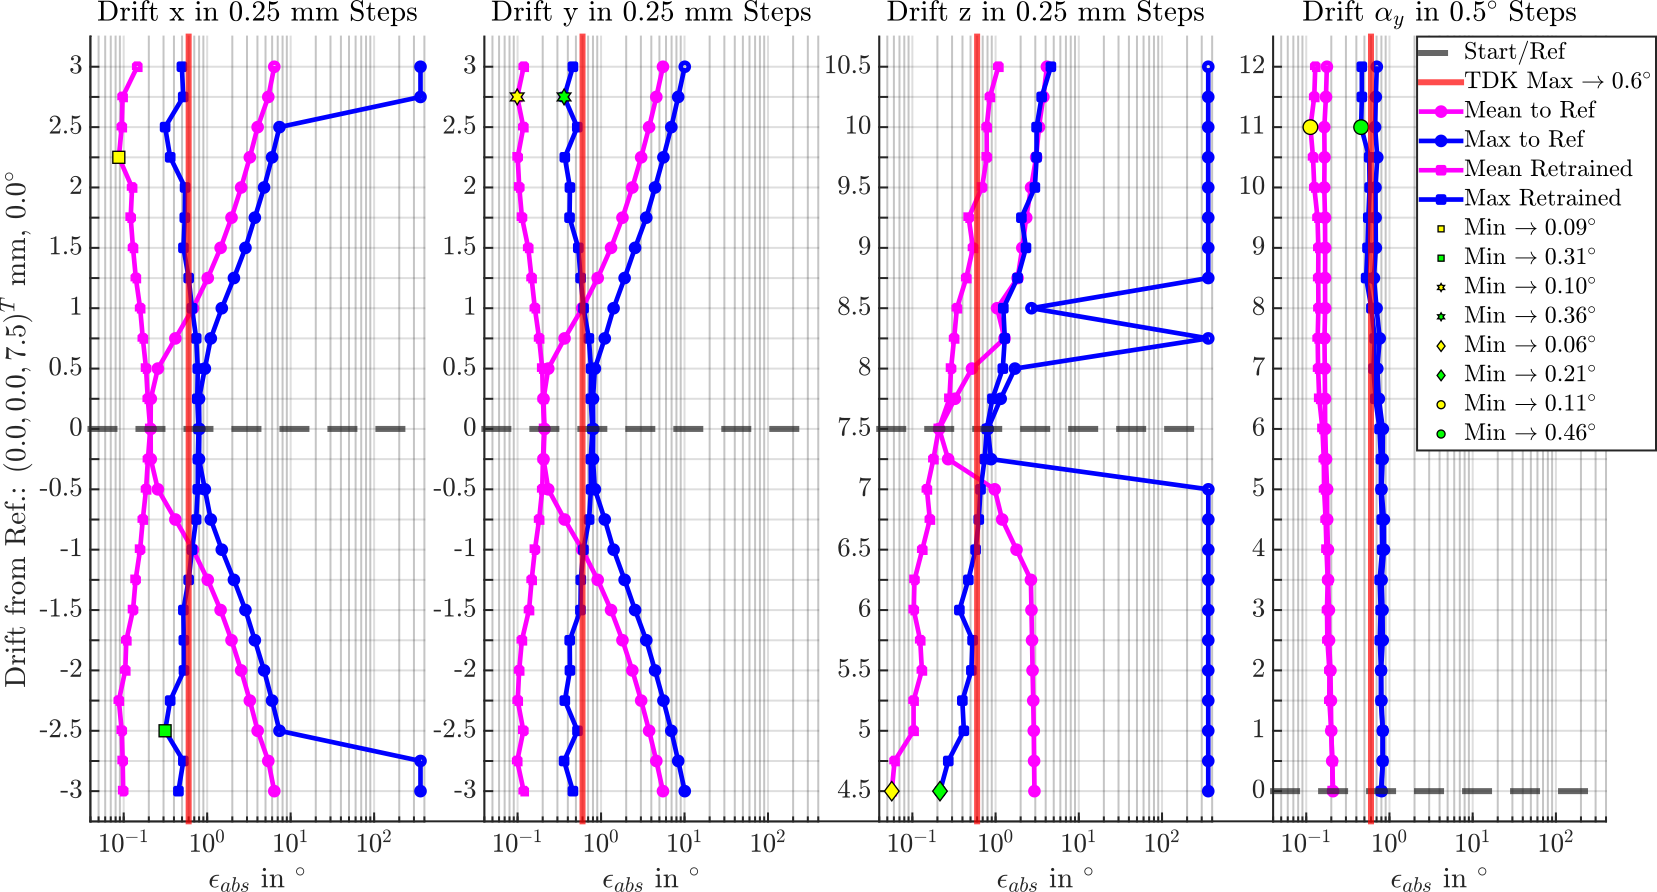
\includegraphics[width=\linewidth]{chapters/images/4-EuOExp/Drift-Model-Errors}
	\caption[Drift xyz tilt mean max errors 2 ref and retrained]{Drift xyz tilt mean max errors 2 ref and retrained}
	\label{fig:drift-model-errors}
\end{figure}
\end{landscape}


\clearpage
\begin{landscape}
\begin{figure}[tbph]
	\centering
	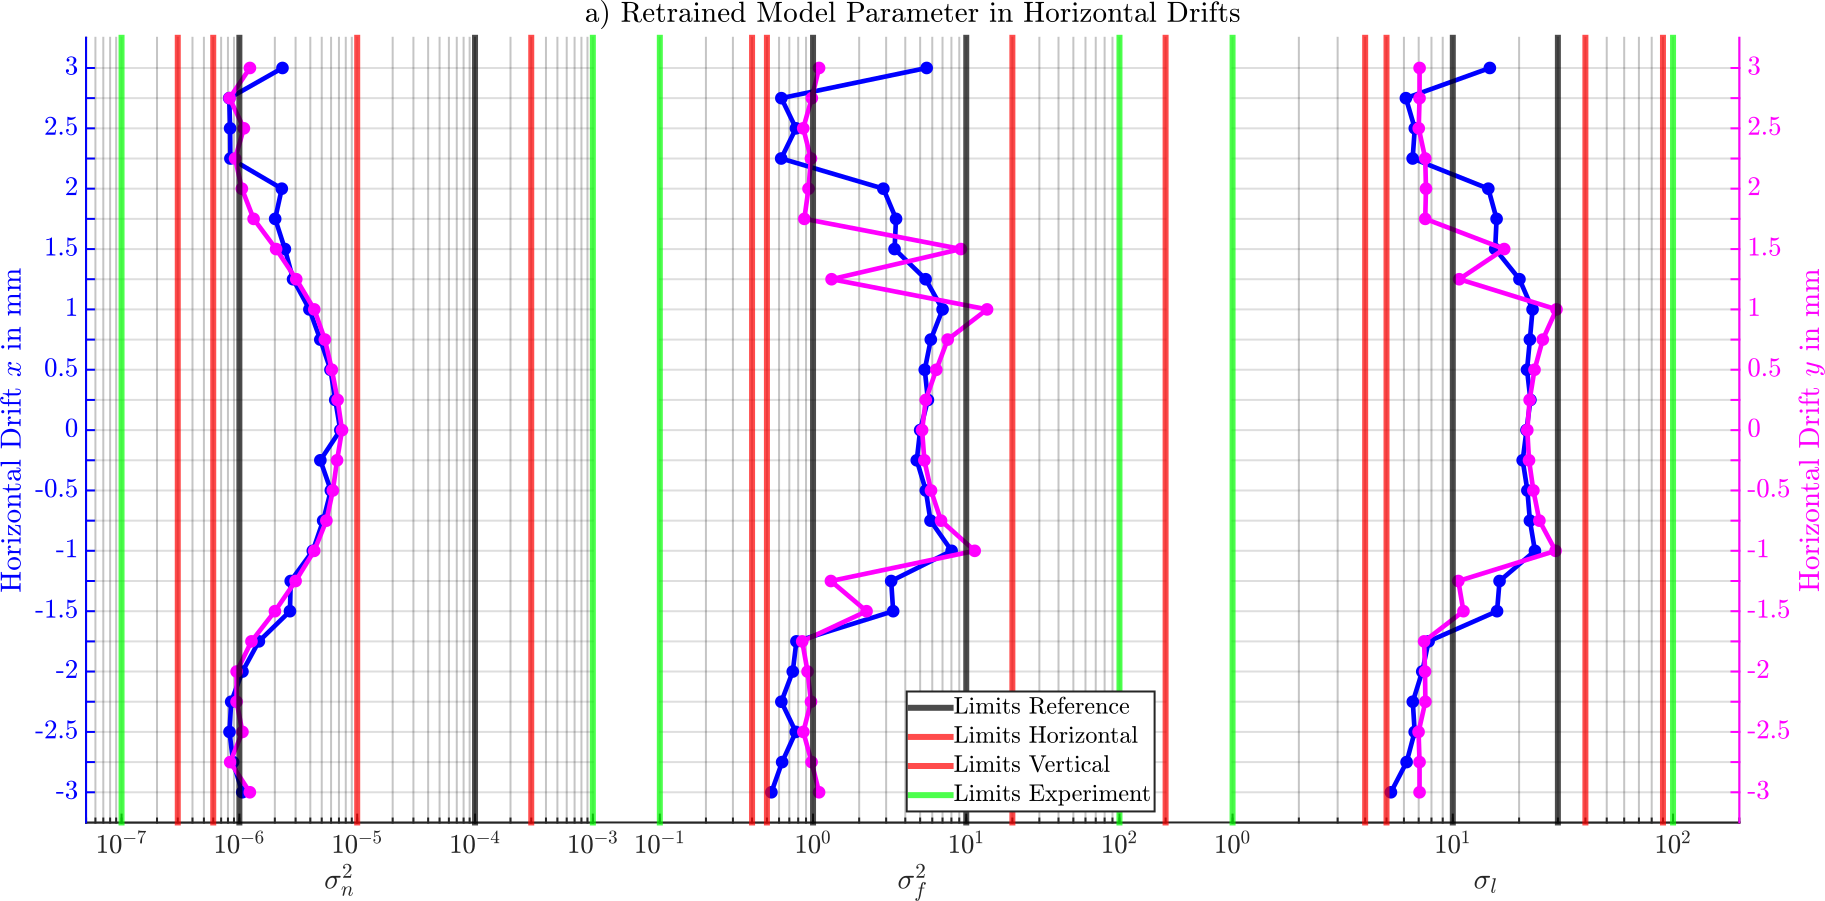
\includegraphics[width=\linewidth]{chapters/images/4-EuOExp/Drift-Horizontal-Model-Parms}
	\caption[Drift xyz tilt retrained model params tracking]{Drift xy retrained model params tracking, limits from exp and ref and new suggestion}
	\label{fig:drift-horizontal-model-parms}
\end{figure}
\end{landscape}

\clearpage
\begin{landscape}
	\begin{figure}[tbph]
		\centering
		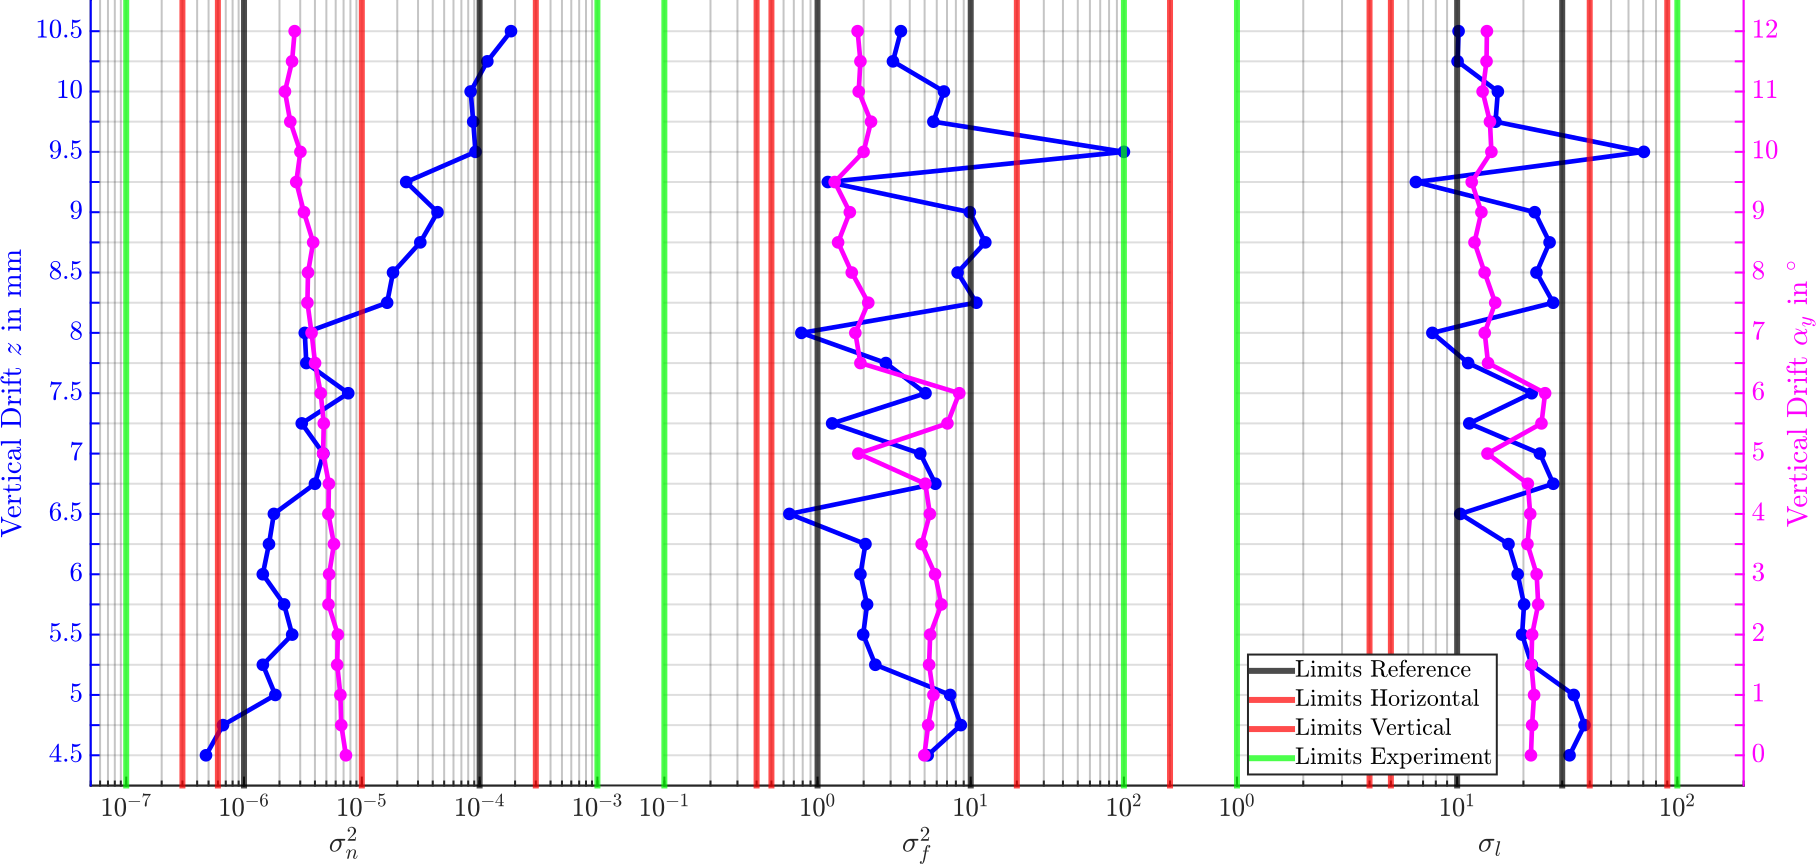
\includegraphics[width=\linewidth]{chapters/images/4-EuOExp/Drift-Vertical-Model-Parms}
		\caption[Drift xyz tilt retrained model params tracking]{Drift z tilt retrained model params tracking, limits from exp and ref and new suggestion}
		\label{fig:drift-vertical-model-parms}
	\end{figure}
\end{landscape}

\clearpage
\begin{figure}[tbph]
	\centering
	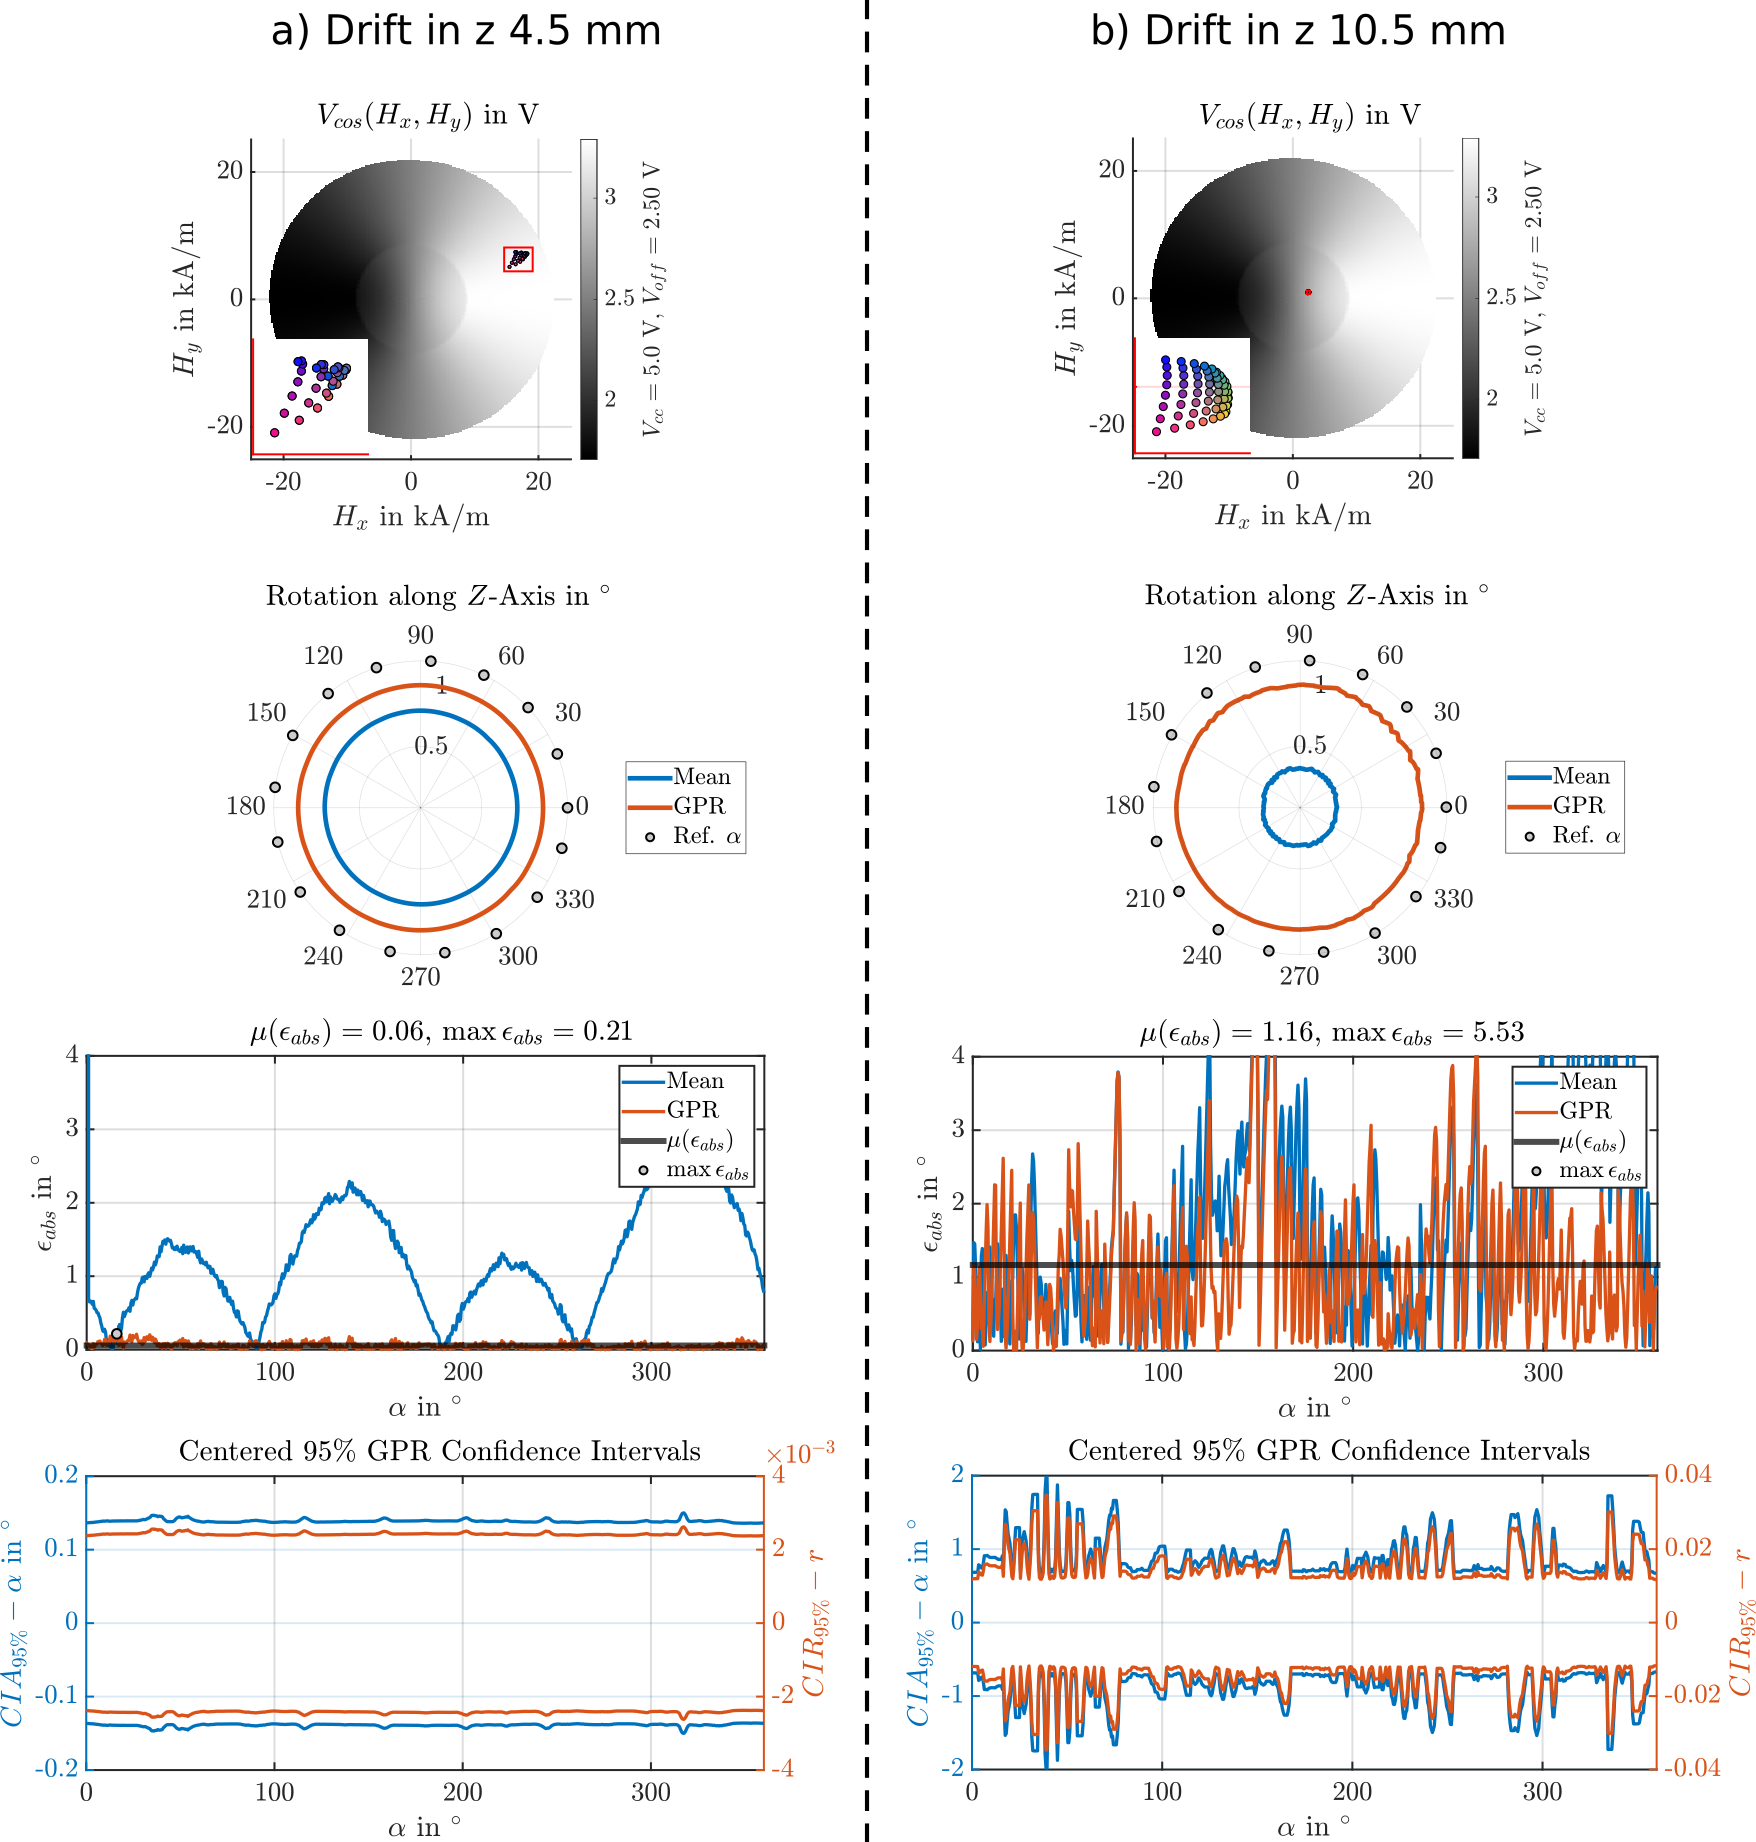
\includegraphics[width=\linewidth]{chapters/images/4-EuOExp/Z-Pos-Comp-45-105-Rotation}
	\caption[Zpos 45 105 comp rotation]{Zpos a) 45 b) 105 comp rotation $\SI{21,5}{\degree}$ comp char spredding}
	\label{fig:z-pos-comp-45-105-rotation}
\end{figure}


\clearpage

